%PREAMBLE____________________________________________________________
\documentclass[a4paper,12pt,onecolumn,twoside]{article}

%Math and symbol packages
\usepackage{amsmath}
\usepackage{amsfonts}
\usepackage{amssymb}
\usepackage{deluxetable}

%Graphics
\usepackage{graphicx}
\usepackage{grffile} %Allows the graphics files to have spaces in their addresses
\usepackage{caption}
\usepackage{subcaption}
\graphicspath{{figs/}}

%Fonts
%\usepackage{fontspec}% Allows choosing font from the local font library
%\defaultfontfeatures{Mapping=tex-text}
%\setmainfont[SmallCapsFont = Fontin SmallCaps]{Fontin}
%\usepackage{titlesec} for customizing section headers

%Page setup
\usepackage[left = 0.5in, right = 0.5in, top = 0.8in, bottom =1in]{geometry}
\usepackage[colorlinks=true, linkcolor = blue, citecolor = blue]{hyperref}%Coloured hyperlinks
\setlength{\columnsep}{0.3in} %column separation

%____________________________________________________________________

%DOCUMENT_________________________________________________________
%Spellcheck
%!TeX spellcheck = en-GB
\begin{document}
%---------------------------------------------------
	\title{Industrial lecture report}
	\author{H. S. Sunil Simha \\\small PH13B011}
	\date{Jul-Nov 2017}
    \maketitle
%-------------------------------------------------- 
\section{Introduction}
This report is based on the seminars and colloquia held at the Department of Physics. I have found the following topics interesting and thus have compiled a brief report on the contents discussed in a particular talk on the detection of the binary neutron star system merger by both electromagnetic and gravitational wave detectors.
\section{Multimessenger astrophysics}
This talk by Dr. Chandrakant Mishra was based on the recent paper by the LIGO and Virgo collaborations \cite{Abbot2017}. This paper discusses the observation of a binary neutron-star inspiral through the LIGO interferometer and the subsequent follow-up observation of a gamma-ray burst by the Fermi-GBM telescope.
	\subsection{GW detection}
		The event of interest was observed on the 17th of August 2017. The inspiral signal, GW170817, was detected by the LIGO telescopes at Hanford and Livingston. Interestingly, their European counterpart (Virgo) did not detect the event and this non-detection proved to be crucial to the localization and quick follow-up via electromagnetic scopes.
		\subsubsection{Glitch removal}
			\begin{figure*}[t]
				\begin{subfigure}{0.45\textwidth}
					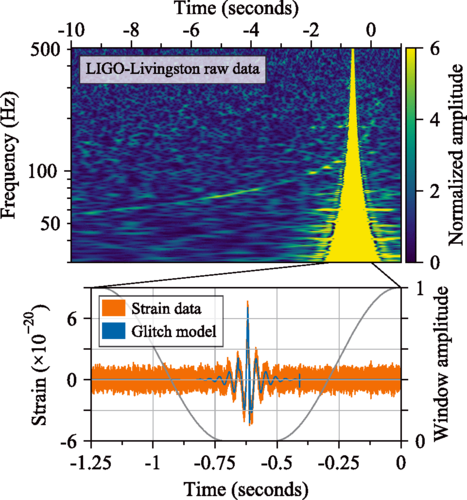
\includegraphics[width=\textwidth]{glitch.png}
					\caption{}
					\label{fig:glitch}
				\end{subfigure}
				\begin{subfigure}{0.45\textwidth}
					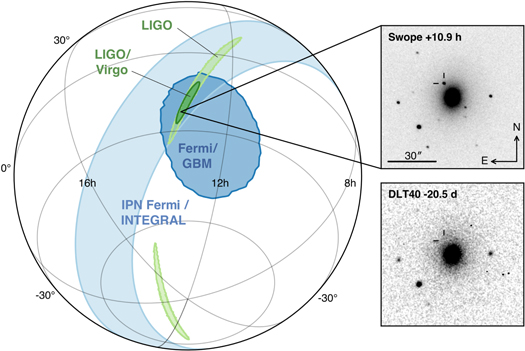
\includegraphics[width=\textwidth]{localization.png}
					\caption{}
					\label{fig:localize}
				\end{subfigure}
				\caption{\footnotesize \textit{Left Top figure:} The instrumental glitch observed just 1.1 seconds before the merger. \textit{Left Bottom figure:} Modelling the glitch and its subtraction. \textit{Source: B. P. Abbot et al, Phys. Rev. Lett., 119, 161101}. \textit{Right figure:} Localization of the source. The large band essentially comes from the non-detection by Virgo. The images on the right show NGC 4993 before and after the event, clearly demarcating the source. \textit{Source: B. P. Abbot et al, Astr. J. Lett., 848: L12 (59pp)}}
			\end{figure*}
			The Livingston data was initially marred by an instrumental glitch (see fig. \ref{fig:glitch}). A noise transient was observed just 1.1 seconds before the merger. Such events are regularly detected on both LIGO instruments and they are uncorrelated and essentially local phenomena. Fortunately, it is a simple matter of modelling the glitch and subtracting it from the data.
			
		\subsubsection{Signal localization}
			The signal was estimated ot originate around 40 Mpc away, well within the ranges of Hanford (218 Mpc), Livingston (107 Mpc) and Virgo (58 Mpc). However, the Virgo detector could not see it because the signal was in the plane of its arms. This non-detection therefore pinned the signal down to a narrow band in the sky (see fig. \ref{fig:localize}) and therefore effectively reducing the sky area to be searched to 31 sq. degrees as compared to the nearly 200 sq. degree area localised by the LIGO detectors alone.
	\subsection{EM observation}
		Prompt messages were sent out to the electromagnetic partner telescope to search for a viable counterpart in that area. Indeed, 1.7 seconds later, a gamma ray burst was observed by the Fermi-GBM telescope. Further broadband  observations showed the signal in X-ray, UV, optical, IR and radio frequencies \cite{Abbot2017-EM}, thus making the chance of the GW and the electromagnetic signals being uncorrelated very small.
	\subsection{System properties}
		To infer the compactness and hence the nature of the objects in the binary system, one may first start with the masses of the objects. One can rule out binary white dwarfs by simply noting the frequency range of operation is too high for these events. The best mass estimates are 1.36-2.26 solar masses and 0.86-1.36 solar masses \cite{Abbot2017}. These are consistent binary systems having neutron stars. However, gravitational waves alone cannot rule out the possibility of even more compact sources.
		
		Electromagnetic observations \cite{DroutShappee2017} showed a power-law and a blue, featureless continuum between 5000 and 10000 $\AA$ which is uncommonly found in young core-collapse supernovae and cataclysmic variable stars. Further observations during the next day showed a rapid fall-off of intensity and also a lack of line absorption features as one would expect of a supernova remnant.
	\subsection{Implications}
		\subsubsection{Neutron star EoS}
			The energy of the gravitational waves depends critically on the equation of state of the neutron stars. Tidal deformability parameters obtained from the data favoured models that predict more compact objects. This could potentially rule out models such as MS1.
		\subsubsection{Fundamental physics}
			The delay in the arrival of EM signals can be mostly attributed to the dynamics of their generation. Such a short gap in the times of arrival lays very strong constrains on the difference in the speeds of the EM and GW propagations. Theoretically, there is supposed to be none. If one were to assume the two signals originated simultaneously, the difference in speeds then must be less than one part in $10^{16}$. This is simply because the signals travelled 40 Mpc.
		\subsubsection{GRBs}
			Having identified the source of the gamma ray burst as a NS-NS merger, one can infer that at least a subset of short GRBs must originate from such activity. The delay time also hints at the possible models of the cataclysmic event and the subsequent generation of electromagnetic radiation. While a single merger is not sufficient to constrain the models a lot, future studies and observations of similar phenomena can improve bounds.
		\subsubsection{Cosmology}
			GWs provide an independent measure of the luminosity distance of the source. Combining this with the redshift measurement of the source, which was identified to have come from NGC 4993, one can get an estimate of the Hubble parameter. Using this method, it was possible to measure $H_0=70^{+12}_{-8}km/s/Mpc$. While this is not such a great measurement by itself, it is consistent with Planck. More such signals will improve these bounds.
\begin{thebibliography}{10}
    \bibitem{Abbot2017} \textbf{B. P. Abbot et al}, 2017, \textit{Phys. Rev. Lett.} 119, 161101
    \bibitem{Abbot2017-EM} \textbf{B. P. Abbot et al}, 2017, \textit{Astr. J. Lett.}, 848:L12 (59pp)
    \bibitem{DroutShappee2017}
    \textbf{M. R. Drout, J. D. Simon, B. J. Shappee et al}, 2017a GCN 21547
\end{thebibliography}

\end{document}